\chapter{Pacote ROS (cliente)}\label{cap:cliente}

Como já foi mencionado anteriormente, o cliente é um pacote ROS, sendo assim, deve-se levar em consideração os conceitos de programação do framework ROS em seu desenvolvimento. As técnicas específicas de programação ROS usadas no cliente serão descritas com detalhes neste capítulo, além da explicação do seu funcionamento interno e do uso da libinterfacesocket.

No desenvolvimento de aplicações com ROS deve ser respeitada a estrutura de diretórios  de um pacote ROS\@. Pacotes são a maneira com que os softwares são organizados no ROS, eles podem conter desde nós, que são a unidades de processamento do ROS, até mesmo bibliotecas ou módulos de softwares de terceiros. Os pacotes devem seguir uma estrutura padrão, por este motivo o código fonte do cliente foi organizado como é mostrado na Imagem~\ref{fig:clientdiretorios}.

\begin{figure}[ht]
	\caption{Estrutura de diretórios pacote cliente}
	\begin{center}
		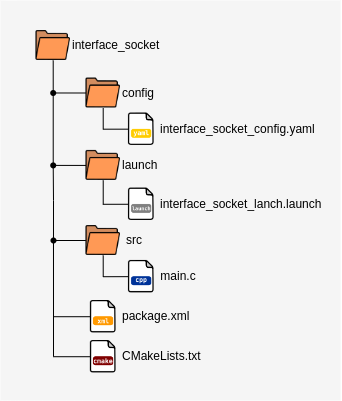
\includegraphics[scale=0.42]{imagens/rospackage.png}\\
		{\small \textbf{Fonte:} do autor}
    \end{center}\label{fig:clientdiretorios}
\end{figure}

A seguir será apresentada uma breve descrição de cada item do pacote:
 
\textbf{config/interface\underline{\hspace{.07in}}socket\underline{\hspace{.07in}}config.yaml:} Arquivo com o qual o usuário pode mudar alguns parâmetros de configuração da comunicação, como IP do servidor ou alguns outros parâmetros do tópico que será lido, como pode ser visto na Figura~\ref{fig:codigoconfig}. Essa mudança pode ocorrer sem a necessidade de recompilar o código fonte, o que pode dar flexibilidade ao usuário do pacote durante o desenvolvimento de uma nova aplicação, que poderá ser configurada sem alterações no código fonte do nó. 

\begin{figure}[ht]
\caption{Configurações do cliente}
\begin{center}
\begin{lstlisting}[language=C++, backgroundcolor=\color{gray!10}]
 server_ip: "127.0.0.1"
 port: 4242

 fps: 15
 encoding: "rgb8"
 height: 720
 width: 1280
 step: 3840
 header.frame_id: "camera_link"
\end{lstlisting}
{\small \textbf{Fonte:}Elaborado pelo autor}	
\end{center}\label{fig:codigoconfig}
\end{figure}
	

\textbf{launch/interface\underline{\hspace{.07in}}socket.launch:} Arquivo responsável chamar a execução do nó, além de carregar os parâmetros presentes no arquivo config.yaml no servidor de parâmetro do ROS\@.

\textbf{src/main.cpp:} Código fonte do executável, ou seja, o código fonte do nó presente neste pacote.

\textbf{package.xml:} Manifesto do pacote é o arquivo que define as propriedades do pacote, como por exemplo, nome do pacote, autor, e dependências. Deve estar presente em todos os pacotes ROS~\cite{RosPkgXml}.


\textbf{CmakeLists.txt:} Contém instruções e diretivas para configuração do processo de compilação do pacote.

O pacote cliente disponibiliza apenas um executável, ou seja, apenas um nó. Assim que o no é executado ele realiza a requisição para estabelecer a conexão com o servidor: com a conexão estabelecida o cliente pode dar início à sua função, ler dados de um tópico e enviá-los ao servidor. Antes de serem enviados ao servidor, os dados precisam ser preparados: informações importantes para o funcionamento interno do ROS, como campos dos cabeçalho, ou timestamp das mensagens, não serão enviados ao servidor. Ou seja, apenas os dados brutos são enviados, contribuindo para a diminuição de dados trafegando na rede.

\begin{figure}[ht]
\caption{Função Callback para o tópico lido pelo cliente}
\begin{center}
\begin{lstlisting}[language=C++, backgroundcolor=\color{gray!10}]
 // Variavel que armazena apenas os dados contidos no 
 // topico lido pleo cliente
 std::vector<uint8_t> dados_out(MSG_LEN);
 
 void image_rawCallback 
 		(const sensor_msgs::Image::ConstPtr & image){
 	// Apenas o campo data he armazenado na variavel
 	dados_out = image->data;
 }

\end{lstlisting}
{\small \textbf{Fonte:}Elaborado pelo autor}	
\end{center}\label{fig:codreaddata}
\end{figure}
		

Após os dados serem enviados ao servidor, o cliente deve ser capaz de recebê-los assim que o servidor atender à requisição. Neste ponto os dados já foram processados pelos circuitos do FPGA, mas como apenas os dados brutos foram enviados ao servidor, o cliente precisa montar novamente a mensagem, disponibilizando os dados processados a partir do tópico de saída, para que os outros nós do sistema possam utilizar esses dados em suas funcionalidades. O processo descrito anteriormente é relativamente simples, como pode ser visto no fluxograma simplificado da Figura~\ref{fig:clientfluxo}


\begin{figure}[ht]
	\caption{Fluxograma pacote cliente}
	\begin{center}
		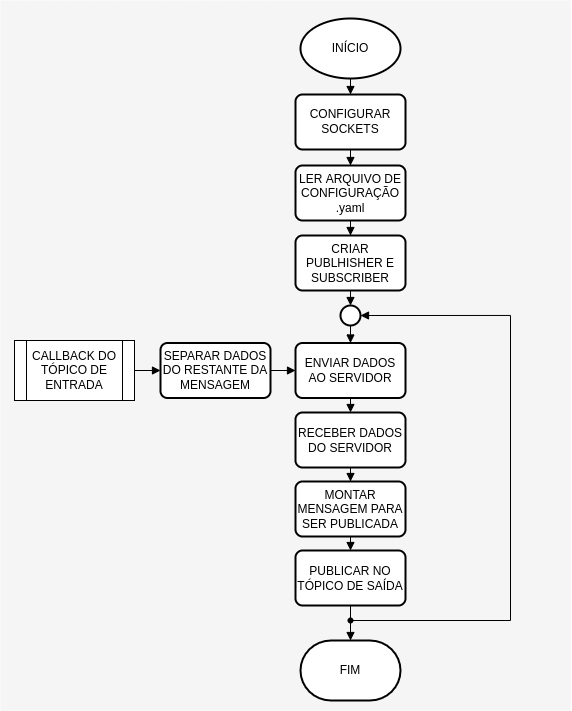
\includegraphics[scale=0.47]{imagens/fluxogramaCliente.png}\\
		{\small \textbf{Fonte:} do autor}
    \end{center}\label{fig:clientfluxo}
\end{figure}


\section{Outras alternativas}

Se seu objetivo for apenas estabelecer a comunicação entre dois dispositivos, já existe um pacote ROS pronto que atenderá a sua necessidade. O \textit{ROS serial} é uma pacote que tem como principal objetivo permitir a comunicação entre o ROS e outro dispositivo que possua uma porta serial ou uma interface de rede~\cite{RosSeria}. Sendo assim o ROS serial seria uma opção genérica, que não depende do dispositivo de hardware. Além do ROS serial, foi encontrado um trabalho em que os autores estabeleceram a comunicação entre o ROS e um FPGA\@. 

A grande diferença deste trabalhos para o proposto é a busca por No trabalho de Yamashina et al. (2005), são demonstradas três técnicas para realizar a conexão entre o FPGA e o ROS, que se diferem da proposta por essa pesquisa. A escolha por desenvolver um novo pacote para executar a mesma função se fez necessário pela necessidade de alta taxa de transferência de dados entre o ROS e o SoC para que seja aceitável a utilização do SoC com a finalidade de acelerar o processamento por hardware. 

Desenvolvendo um novo pacote de comunicação podemos extrair o máximo de desempenho da rede, como por  xemplo, escolhendo o melhor protocolo (UDP ou TCP) e transferindo apenas os dados para o processamento da informação. Todos os códigos do cliente podem ser encontrados no repositório disponível em~\cite{interface-socket}.
